% Background: technical_background sec 4 (kappa(s) and the noise problem). The turning angle and its
% atan2 form are defined HERE, not in the background (user, 2026-10-07).
% Technical computation only; the per-artery path is defined in sec:method-split (user, 2026-10-20).
% Only this feature: the general feature introduction is in 05_features.tex (user, 2026-11-06).
% Register after Aida Ch. 5 (style_guide_methodology_aida.md): past passive, where-sentences, reasons.
% Implementation: CGPS_data/thesis_final/turning_feature.py (mean_turning, segment_turning), which runs
%   profile_thesis of tortuosity/curvature.py (sliding window, smooth=0) on each trunk of split_trunks.
% Figure: turning_feature_schematic.py (made-up trunk, run through the same code).
% The FPCA of the profile (pLAD, mLAD) and its 50-point grid are a secondary analysis, in
% 07_curvature_fpca.tex (sec:method-fpca).
% TODO: confirm that the tracer centerlines arrive smoothed; the text says no extra smoothing (smooth=0).
%   The question to Kit is the \clarify note in 01a_inhouse_tracer.tex.
% 2026-11-06 rewrite (thesis-style, Aida register, for a first read): one job per paragraph in the
%   order of the computation (angle, chord length, profile, segment mean, origin). Heading to
%   sentence case. Plain-words definition of the turning angle added before the equation.
% Cut as already said earlier: why mean curvature rather than the tortuosity index (kashyap2022:
%   literature review and sec:method-selection); what Tello Ayala et al. computed (literature
%   review), so the last paragraph now states only how this feature differs from theirs.
% 2026-11-06 (user): opens on "quantified as mean turning angle" with a one-clause pointer back to
%   kashyap2022 in the literature review (average curvature most closely related to low WSS).
%   CAREFUL: kashyap is a simulation study of the LM bifurcation in CAD-free individuals and the
%   relation was weak; keep "although weakly", do not upgrade to "predicts plaque".
% 2026-11-06 (user: concise and academic): condensed to three paragraphs; plain-words gloss of the
%   turning angle, the start-independence sentence and the closing pointer to sec:method-models cut;
%   eq:method-profile kept, as 07_curvature_fpca.tex refers to it.
% Wording: sigma/l^2 noise fact kept as "falls with the square of the chord length".
\subsection{Turning-angle curvature}
\label{sec:method-curvature}

Curvature was quantified as the mean turning angle per millimeter, a form of the average curvature, which was the tortuosity measure most closely, although weakly, related to low WSS (Chapter~\ref{ch:literature}) \cite{kashyap2022tortuosity}.
The turning angle $\theta_i$ at centerline point $\mathbf{P}_i$ was measured between two chords of fixed length $\ell = 5$\,mm, so that every angle spans the same length of vessel despite the uneven point spacing (Figure~\ref{fig:method-turning}).
The chord ends $\mathbf{B}_i$ and $\mathbf{F}_i$ lie 5\,mm before and after $\mathbf{P}_i$ in a straight line and were found by linear interpolation between neighboring centerline points.
To retain precision for nearly straight vessels, where the cosine of the angle is close to 1, the angle was computed as
\begin{equation}
  \theta_i = \operatorname{atan2}\bigl(\lVert \mathbf{a}_i \times \mathbf{b}_i \rVert,\; \mathbf{a}_i \cdot \mathbf{b}_i\bigr),
  \qquad \mathbf{a}_i = \mathbf{P}_i - \mathbf{B}_i,\quad \mathbf{b}_i = \mathbf{F}_i - \mathbf{P}_i ,
  \label{eq:method-turn}
\end{equation}
where $\mathbf{a}_i$ and $\mathbf{b}_i$ are the arriving and leaving chords, and $\theta_i \in [0, \pi]$ is unsigned, as each bend of a 3D vessel lies in its own plane.

A positional error $\sigma$ in the centerline tilts a chord by about $\sigma/\ell$, so the spurious turning per millimeter decreases with $\ell^2$.
The 5\,mm chord, previously used for coronary curvature on CCTA \cite{vanzandwijk2019curvature}, limits this error at the cost of not resolving bends shorter than a few millimeters.
No further smoothing was applied, and points within 5\,mm of either end of the artery were assigned no value.

The curvature profile,
\begin{equation}
  \kappa_i = \frac{\theta_i}{\ell} ,
  \label{eq:method-profile}
\end{equation}
in rad/mm, was computed along the whole artery (Section~\ref{sec:method-split}) and then divided at the segment boundaries, so that angles near a boundary use chords extending into the neighboring segment.
To avoid overweighting densely sampled stretches, each segment $s$ was summarized by the arc-length mean of its profile,
\begin{equation}
  T_s = \frac{1}{s_{\mathrm{last}} - s_{\mathrm{first}}} \int_{s_{\mathrm{first}}}^{s_{\mathrm{last}}} \kappa(s)\,\mathrm{d}s ,
  \label{eq:method-tl}
\end{equation}
where $s_{\mathrm{first}}$ and $s_{\mathrm{last}}$ are the arc lengths of its first and last profile point.
The integral was evaluated with the trapezoid rule, and segments with fewer than two profile points were recorded as missing.
The feature is adapted from the turning-angle score of Tello Ayala et al.\ \cite{telloayala2026tortuosity}, which averages angles between consecutive points of 2D angiographic centerlines; here the centerlines are 3D, the chord is fixed and the turning is normalized by length, so $T_s$ is independent of the point spacing.

% Figure from turning_feature_schematic.py (made-up trunk, no patient data).
\begin{figure}[htbp]
  \centering
  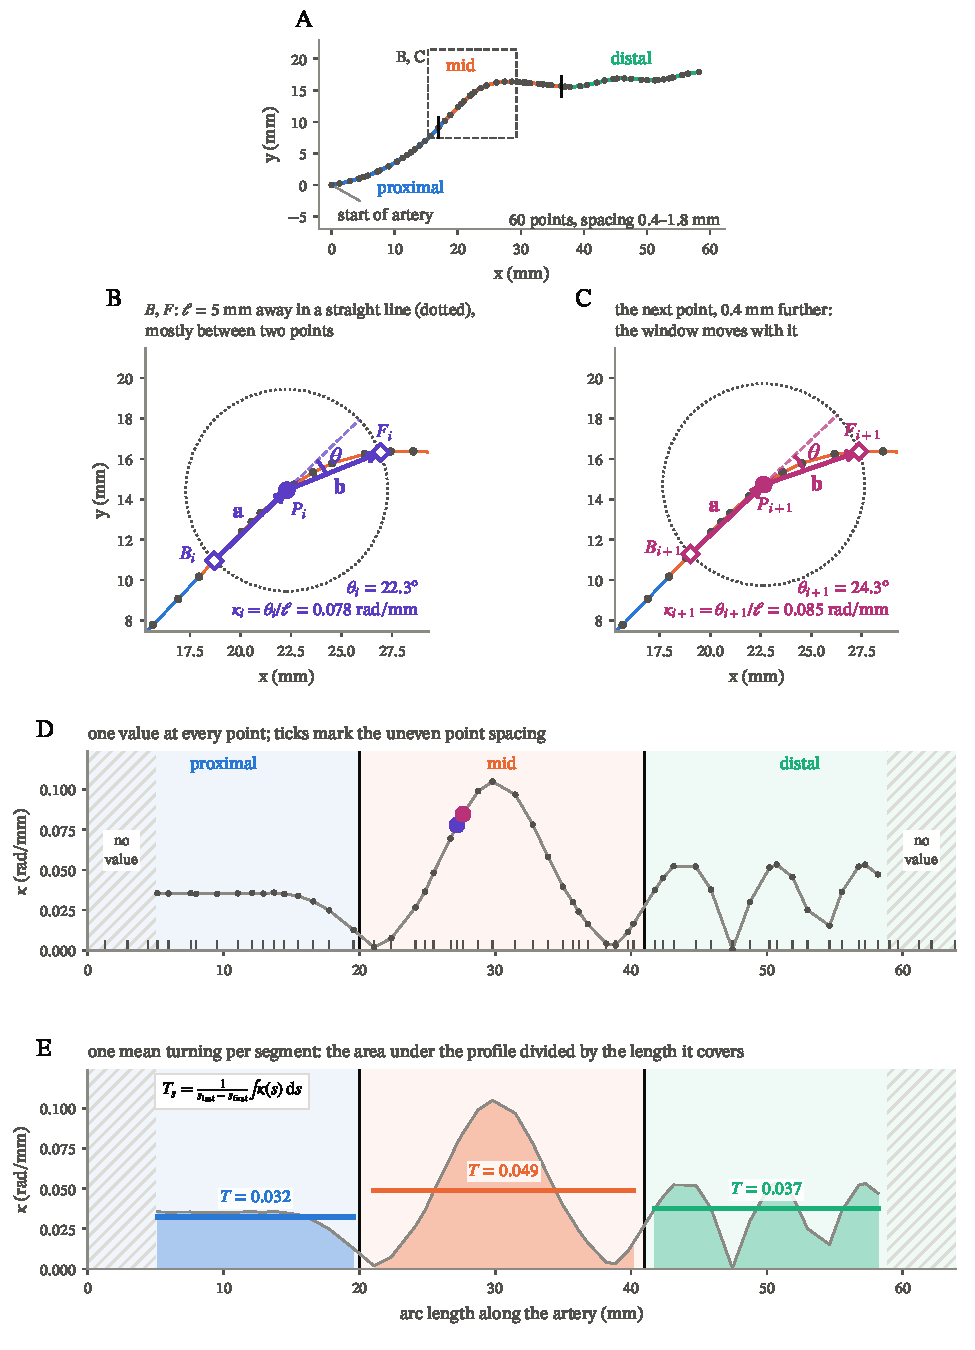
\includegraphics[width=\textwidth]{methodology/turning_feature_schematic.pdf}
  \caption{From centerline points to one mean curvature per segment, on a made-up artery with unevenly spaced points (dots) and made-up segment boundaries (black ticks). (A) The artery, divided into a proximal, a mid and a distal segment. (B) At point $P_i$, the points $B_i$ and $F_i$ (diamonds) lie 5\,mm away in a straight line (dotted circle), mostly between two centerline points; $\theta$ is the angle between the arriving chord $\mathbf{a}$, continued straight (dashed), and the leaving chord $\mathbf{b}$. (C) The same at the next point, with its own chords. (D) The curvature profile $\kappa = \theta/\ell$ at every point; the ticks on the axis mark the point spacing, and the first and last 5\,mm (hatched) have no value. (E) The mean curvature $T_s$ of each segment, the area under its profile divided by the length the profile covers, in rad/mm.}
  \label{fig:method-turning}
\end{figure}
